\documentclass{beamer}
\usepackage[utf8]{inputenc}
\usepackage{tabularx}
\usetheme{Frankfurt}
\newcommand\TestAppExists[3]{#2}
\usepackage{minted}
\usepackage{listings}
\usepackage{media9}

\usepackage{pgf}
\usepackage{tikz}
\usetikzlibrary{arrows,automata}
\usepackage{tikz-cd}
\usetikzlibrary{positioning}

   
\usepackage{mathpartir}
\usepackage{multicol}
\usepackage{graphicx}


\lstset{ %
	basicstyle=\small\ttfamily,
	breakatwhitespace=true,
	breaklines=false,
	commentstyle=\color{green!40!black},
	extendedchars=true, 
	keepspaces=true, 
	keywordstyle=\color{blue},
	showspaces=false,               
	showstringspaces=false,         
	showtabs=false,
	tabsize=2
}
  
  \setbeamerfont{institute}{size=\fontsize{7pt}{8pt}}
  
  \title{Copilot : Traceability and Verification of a Low Level Automatically Generated C Source Code}
  \author{Georges-Axel Jaloyan}
  \institute{\'Ecole Normale Sup\'erieure, NASA Langley Research center, National Institute of Aerospace}
  \date{September 9, 2015}
  
\begin{document}
\begin{frame}
  		
  		\titlepage
  		\begin{center}
  			\includegraphics[height=2cm]{images/ENS-logo.jpg} \includegraphics[height=2cm]{images/NASA.png}
  			\includegraphics[height=2cm]{images/NIA-logo.jpg}
  		\end{center}
\end{frame}
  	
  	
  	\section{Preliminaries}
  	\subsection{Copilot language}
\begin{frame}
  		\tableofcontents[currentsubsection,sectionstyle=show/shaded,subsectionstyle=show/shaded/hide]
\end{frame}
  	
\begin{frame}
  		\frametitle{Copilot language}
  		Copilot is an \emph{EDSL} (embedded domain specific language), embedded in \emph{Haskell} and used for writing \emph{runtime monitors} for hard real-time, distributed, reactive systems written in C. 
  		\\~\\
  		\text{A Copilot program, can either be : } 
  		\begin{itemize}
  			\item compiled to C using two back-ends : SBV, ATOM
  			\item interpreted
  			\item analyzed using static analysis tools (CBMC, Kind)
  		\end{itemize} 
\end{frame}
  	
\begin{frame}[fragile]
  		\frametitle{Copilot syntax}
  		A program is a list of streams that can be either external  or internal which are defined by mutually recursive stream equations.
  		\\~\\
  		Each stream has a type which can be \texttt{Bool}, \texttt{Int8}, \texttt{Int16}, \texttt{Int32}, \texttt{Int64}, \texttt{Word8}, \texttt{Word16}, \texttt{Word32}, \texttt{Word64}, \texttt{Float}, \texttt{Double}.
  		
\begin{minted}{haskell}
x :: Stream Word16
x = 0
-- x = {0, 0, 0, ...}
y :: Stream Bool
y = x `mod` 2 == 0
-- y = {T, T, ...}
nats :: Stream Word64
nats = [0] ++ (1 + nats)
-- nats = {0,1,2, ..., 2^64-1, 0, 1, ..}  
\end{minted}
\end{frame}
  	
\begin{frame}[fragile]
	\frametitle{Operators}
  		Each operator and constant has been lifted to Streams (working pointwise). \\~\\
  		Two temporal operations working on Streams : 
  		\begin{itemize}
  			\item ++ : which prepends a finite list to a Stream

\begin{minted}{haskell}
(++) :: [a] -> Stream a -> Stream a
\end{minted}
  			\item drop : which drops a finite number of elements at the beginning of a Stream
\begin{minted}{haskell}
drop :: Int -> Stream a -> Stream a  
\end{minted}
  		\end{itemize}
  		
Casts and unsafe casts are also provided :
\begin{minted}{haskell}
cast :: (Typed a, Typed b) => Stream a -> Stream b
unsafeCast :: (Typed a, Typed b) => Stream a -> Stream b
\end{minted}
\end{frame}
  	
\begin{frame}[fragile]
  		\frametitle{Examples}
	Fibonacci sequence :
\begin{minted}{haskell}
fib :: Stream Word64
fib = [1,1] ++ (fib + drop 1 fib) 
-- fib = {1,1,2,3,5,8,13,...,
--       12200160415121876738,
--   /!\ 1293530146158671551,...}
\end{minted}

\end{frame}

\begin{frame}[fragile]
	\frametitle{Interaction}
	Sensors :
	\begin{itemize}
		\item<1|only@1> Sample external variables. 
\begin{minted}{haskell}
extern :: Typed a => String -> Maybe [a] -> Stream a
\end{minted}
Example : 
\begin{lstlisting}[language=C]
unsigned long long int x;
\end{lstlisting}
\begin{minted}{haskell}
x :: Stream Word64
x = extern "x" (Just [0,0..])

x2 = externW64 "x" Nothing
\end{minted}

		\item<2-4> Sample external variables. 
		\item<2|only@2> Sample external arrays. 
\begin{minted}{haskell}
externArray :: (Typed a, Typed b, Integral a) => 
String -> Stream a -> Int -> Maybe [[a]] -> Stream b
\end{minted}
Example : 
\begin{lstlisting}[language=C]
unsigned long long int tab[1000];
\end{lstlisting}
\begin{minted}{haskell}
-- nat = [0] ++ (nats + 1)
x :: Stream Word64
x = externArray "tab" nats 1000 Nothing

x2 = externArrayW64 "tab" nats 1000 Nothing
\end{minted}
	
		\item<3-4> Sample external arrays. 
		\item<3|only@3> Sample external functions. 

\begin{minted}{haskell}
externFun :: Typed a => 
String -> [FunArg] -> Maybe [a] -> Stream a
\end{minted}
Example :
\begin{lstlisting}[language=C]
double sin(double a); //from math.h
\end{lstlisting}
\begin{minted}{haskell}
x :: Stream Double
x = externDouble "x" Nothing

sinx = externFun "sin" [arg x] Nothing
\end{minted}
		
		\item<4> Sample external functions. 
	\end{itemize}
\end{frame}
  	
\begin{frame}[fragile]
  		\frametitle{Interaction}
  		
	Actuators :
  	\begin{itemize}
		\item Triggers : 
\begin{minted}{haskell}
trigger :: 
  String -> Stream Bool -> [TriggerArg] -> Spec
\end{minted}
		\item Observers :
\begin{minted}{haskell}
observer :: Typed a => String -> Stream a -> Spec
\end{minted}
	\end{itemize}
\end{frame}
  	
  	\subsection{ACSL}
  	\begin{frame}
  		\tableofcontents[currentsubsection,sectionstyle=show/shaded,subsectionstyle=show/shaded/hide]
  	\end{frame}
  	
\begin{frame}[fragile]
	\frametitle{ACSL syntax}
	ACSL is a specification language for C programs. Those contracts are written according to the following example :
\begin{lstlisting}[language=C]
/*@ requires true
assigns \nothing
ensures \result >= x && \result >= y;
ensures \result == x || \result == y;
*/
int max (int x, int y) { return (x > y) ? x : y; }
\end{lstlisting}
	
\end{frame}


\begin{frame}[fragile]
\begin{figure}[ht!]
	\centering
	\footnotesize
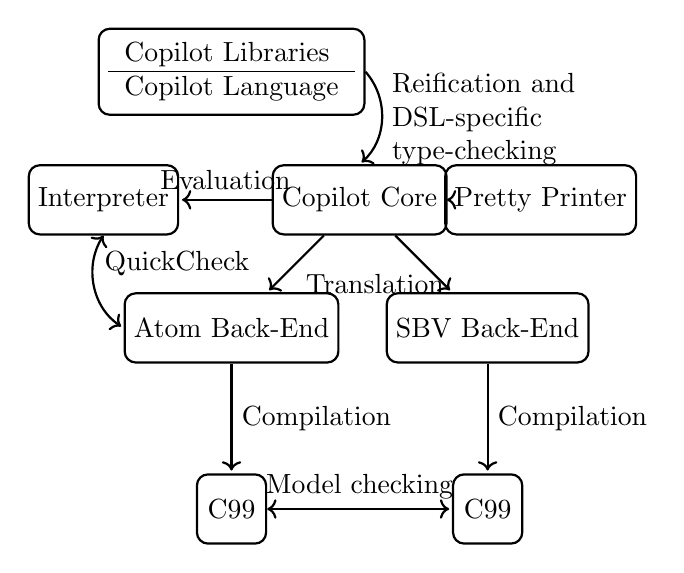
\begin{tikzpicture}[->, node distance=2.3cm, auto, shorten >=1pt, bend angle=45,thick]
\tikzstyle{every state}=[rectangle, rounded corners]
	
	
\node[state] (Int) {Interpreter};
\node[state] (Lang) [above right of=Int]
{
	\begin{tabular}[b]{l}
	Copilot Libraries\\ \hline Copilot Language
	\end{tabular}};
\node[state] (Core) [below right of=Lang] {Copilot Core};
\node[state] (PP) [right of=Core] {Pretty Printer};
		
		
\node[state] (Atom) [below left of=Core] {Atom Back-End};
\node[state] (SBV) [below right of=Core] {SBV Back-End};
\node[state] (C99A) [below of=Atom] {C99};
\node[state] (C99S) [below of=SBV] {C99};
		
		
\tikzstyle{every node}=[]
		
		
\path %% (Libs) edge node {0,1,L} (Lang);
%% edge node {1,1,R} (C)
(Lang) edge [bend left, anchor=west, text width=2.5cm] node {Reification and DSL-specific type-checking} (Core)
%% edge node {0,1,L} (C)
(Core) edge node {Translation} (Atom)
edge node {} (SBV)
edge node {} (PP)
edge node [swap] {Evaluation} (Int)
(Int) edge [<->, bend right] node {QuickCheck} (Atom)
(Atom) edge node {Compilation} (C99A)
(SBV) edge node {Compilation} (C99S)
(C99A) edge [<->] node {Model checking} (C99S);
%% edge [bend left] node {Translation} (SBV)
%% (Atom) edge [loop below] node {1,1,R} (D)
%% edge node {0,1,R} (Libs)
%% (SBV) edge [bend left] node {1,0,R} ();
\end{tikzpicture}
\caption{The Copilot toolchain\footnote{L. Pike, N. Wegmann, S. Niller, and A. Goodloe, \textit{Experience report: A do-it-yourself high-assurance compiler}, 2012.}}
	\end{figure}
\end{frame}
  	
  	  	\section{Working on the backend}
\subsection{}
\begin{frame}
	\tableofcontents[currentsubsection,sectionstyle=show/shaded,subsectionstyle=show/shaded/hide]
\end{frame}


\begin{frame}[fragile]
\frametitle{ACSL generation}
The easiest way to do it is by induction on the syntax, when compiling the expression. Here is how the function ppACSL is constructed :
\begin{itemize}
	\item $\texttt{Const~type~value} \rightarrow show~\texttt{value}$
	\item $\texttt{Drop~type~i~id} \rightarrow queue\_\texttt{id} \lbrack ptr\_\texttt{id} + \texttt{i} ~ mod ~ (length~\texttt{id}) \rbrack$
	\item $\texttt{ExternVar~t~name~b} \rightarrow ext\_\texttt{name}$
	\item $\texttt{Var type name} \rightarrow \texttt{name}$
	\item $\texttt{Op2 op e1 e2} \rightarrow (ppACSL~\texttt{e1})~show~\texttt{op}~(ppACSL~\texttt{e2})$
	\item $\texttt{Label~t~s~e} \rightarrow ppACSL~\texttt{e}$
\end{itemize}
\end{frame}

\begin{frame}[fragile]
\frametitle{ACSL generation}
Nevertheless, some hacks :

\begin{itemize}
	\item Let bindings have been deprecated.
	\item Abs are converted to $\backslash a \rightarrow sign~a \times a$
	\item Sign to $\backslash x \rightarrow ((x > 0)~?~1 : ((x < 0) ? -1 : 0))$
	\item Mux where branches have type Bool to $Mux~e1~e2~e3 = ( e2 \wedge e1) \vee (e3 \wedge \neg e1)$
	\item No bitwise operator are supported.
\end{itemize}
\end{frame}

\begin{frame}[fragile]
	\frametitle{Magic labels}
	The possibility to add labels that would be printed in the C source file was also added in SBV and in Copilot. \\~\\
	The prover was not able to prove long expressions (some were 500000 characters long).\\~\\
	So we need to add a special instruction that has one only role : split the AST into smaller ones that can be easily provable. This instruction has to be totally useless regarding to the semantics of the language. Labels do not change the semantics of the program. So why not using them ? \\~\\
	The idea is to call the function identity when we encounter a magic label. This is equivalent to the transformation : $ e \rightarrow_{\beta} (\lambda x . x) e $. 

\end{frame}

\begin{frame}[fragile]
	\frametitle{Magic labels: example}
\begin{minted}{haskell}
import qualified Copilot.Compile.SBV as S

alt :: Stream Bool
alt = (label "?splitting" $ not $ 
      externB "externvar" Nothing)

spec :: Spec
spec = do
trigger "trigger" (alt) []

main = do
reify spec >>= S.proofACSL S.defaultParams
\end{minted}


\end{frame}

\begin{frame}[fragile]
	\frametitle{Magic labels: example}
	~\\
	\begin{figure}
		\includegraphics[width=33mm]{images/label/main.ps}
		\centering
		\includegraphics[width=33mm]{images/label/splitted.ps}
		\includegraphics[width=33mm]{images/label/splitted2.ps}
	\end{figure}
	
\end{frame}

\begin{frame}[fragile]
	\begin{figure}[ht!]
		\centering
		\footnotesize
		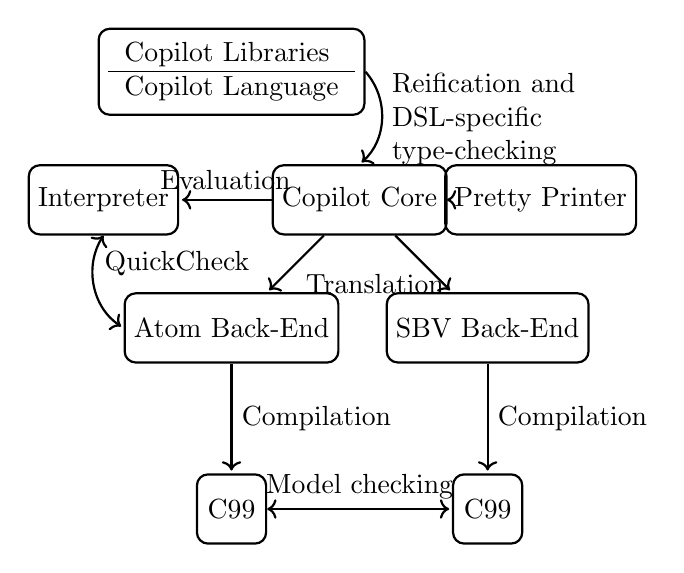
\begin{tikzpicture}[->, node distance=2.3cm, auto, shorten >=1pt, bend angle=45,thick]
		\tikzstyle{every state}=[rectangle, rounded corners]
		
		
		\node[state] (Int) {Interpreter};
		\node[state] (Lang) [above right of=Int]
		{
			\begin{tabular}[b]{l}
			Copilot Libraries\\ \hline Copilot Language
			\end{tabular}};
		\node[state] (Core) [below right of=Lang] {Copilot Core};
		\node[state] (PP) [right of=Core] {Pretty Printer};
		
		
		\node[state] (Atom) [below left of=Core] {Atom Back-End};
		\node[state] (SBV) [below right of=Core] {SBV Back-End};
		\node[state] (C99A) [below of=Atom] {C99};
		\node[state] (C99S) [below of=SBV] {C99};
		
		
		\tikzstyle{every node}=[]
		
		
		\path %% (Libs) edge node {0,1,L} (Lang);
		%% edge node {1,1,R} (C)
		(Lang) edge [bend left, anchor=west, text width=2.5cm] node {Reification and DSL-specific type-checking} (Core)
		%% edge node {0,1,L} (C)
		(Core) edge node {Translation} (Atom)
		edge node {} (SBV)
		edge node {} (PP)
		edge node [swap] {Evaluation} (Int)
		(Int) edge [<->, bend right] node {QuickCheck} (Atom)
		(Atom) edge node {Compilation} (C99A)
		(SBV) edge node {Compilation} (C99S)
		(C99A) edge [<->] node {Model checking} (C99S);
		%% edge [bend left] node {Translation} (SBV)
		%% (Atom) edge [loop below] node {1,1,R} (D)
		%% edge node {0,1,R} (Libs)
		%% (SBV) edge [bend left] node {1,0,R} ();
		\end{tikzpicture}
	\end{figure}
\end{frame}
  	
  	
\begin{frame}[fragile]
	\begin{figure}[ht!]
		\centering
		\tiny
		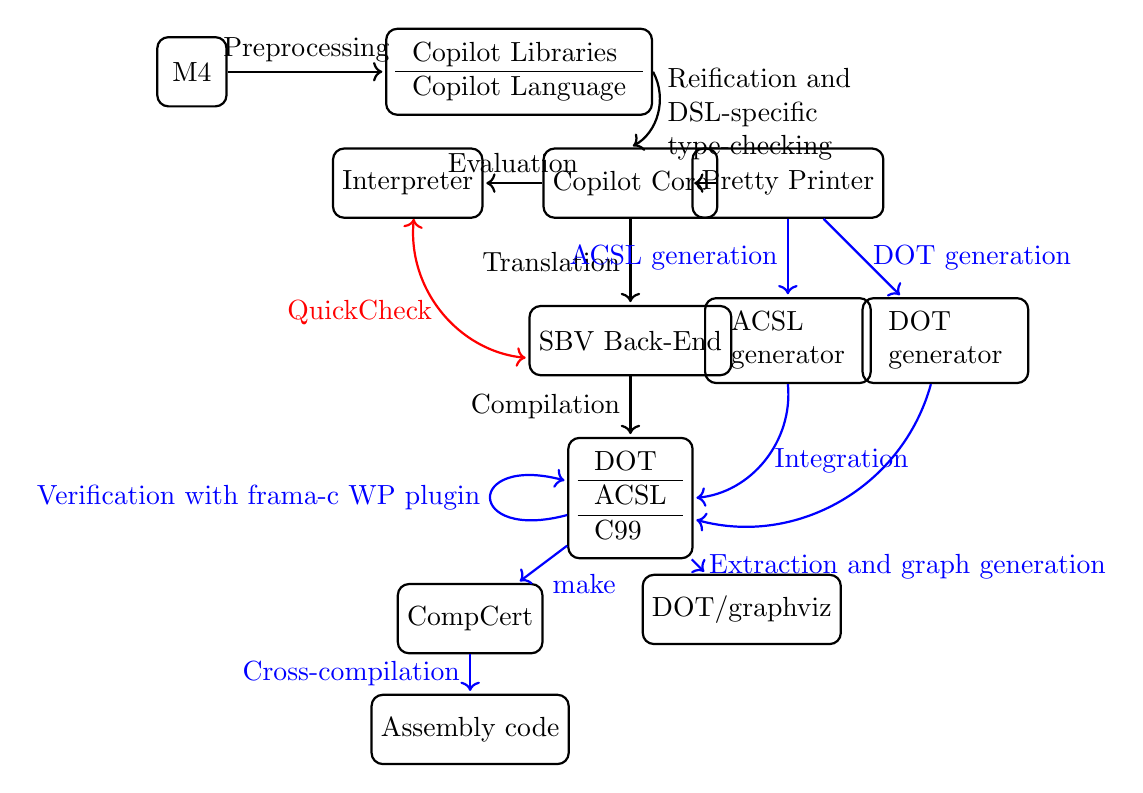
\begin{tikzpicture}[->, node distance=2cm, auto, shorten >=1pt, bend angle=45,
		thick]
		\tikzstyle{every state}=[rectangle, rounded corners]
		
		
		\node[state] (Int) {Interpreter};
		\node[state] (Lang) [above right of=Int]
		{
			\begin{tabular}[b]{l}
			Copilot Libraries\\ \hline Copilot Language
			\end{tabular}};
		
		\node[state] (M4) [left=2cm of Lang] {M4};
		\node[state] (Core) [below right of=Lang] {Copilot Core};
		\node[state] (PP) [right of=Core] {Pretty Printer};
		
		
		\node[state] (ACSL) [below of=PP] {\begin{tabular}[b]{l}
			ACSL\\ generator
			\end{tabular}};
		\node[state] (DOTc) [right of=ACSL] {\begin{tabular}[b]{l}
			DOT\\ generator
			\end{tabular}};
		\node[state] (SBV) [below of=Core] {SBV Back-End};
		\node[state] (C99S) [below of=SBV] {\begin{tabular}[b]{l}
			DOT\\ \hline ACSL\\ \hline C99
			\end{tabular}};
		\node[state] (DOT) [below right of=C99S] {DOT/graphviz};
		\node[state] (CCOMP) [below left=0.3cm and 0.3cm of C99S] {CompCert};
		\node[state] (ASM) [below=0.5cm of CCOMP] {Assembly code};
		
		
		\tikzstyle{every node}=[]
		
		
		\path %% (Libs) edge node {0,1,L} (Lang);
		%% edge node {1,1,R} (C)
		(Lang) edge [bend left, anchor=west, text width=2.5cm] node {Reification and DSL-specific type-checking} (Core)
		%% edge node {0,1,L} (C)
		(M4) edge [] node {Preprocessing} (Lang)
		(Core) edge [anchor=east] node {Translation} (SBV)
		edge node {} (PP)
		edge node [swap] {Evaluation} (Int)
		(ACSL) edge [bend left, anchor=west, blue] node {Integration} (C99S)
		(DOTc) edge [bend left, anchor=east, blue] node {} (C99S)
		(Int) edge [<->,red, bend right, anchor=east] node {QuickCheck} (SBV)
		(PP) edge [->,blue, anchor=east] node {ACSL generation} (ACSL)
		(PP) edge [->,blue, anchor=west] node {DOT generation} (DOTc)
		(C99S) edge [->,blue, anchor=north west] node {make} (CCOMP)
		(CCOMP) edge [->,blue, anchor=east] node {Cross-compilation} (ASM)
		(C99S) edge [loop left, ->,blue, anchor=east] node {Verification with frama-c WP plugin} (C99S)
		(C99S) edge [->,blue, anchor=west] node {Extraction and graph generation} (DOT)
		(SBV) edge [->,anchor=east] node {Compilation} (C99S);
		%% edge [bend left] node {Translation} (SBV)
		%% (Atom) edge [loop below] node {1,1,R} (D)
		%% edge node {0,1,R} (Libs)
		%% (SBV) edge [bend left] node {1,0,R} ();
		\end{tikzpicture}
	\end{figure}
\end{frame}

\begin{frame}[fragile]
	\frametitle{And it works !}
\begin{itemize}
	\item 3 front-end bugs
	\item 1 big back-end bug
\end{itemize}
	
\end{frame}


\section{Applications}
\subsection{Self-separation criteria}
\begin{frame}
	\tableofcontents[currentsubsection,sectionstyle=show/shaded,subsectionstyle=show/shaded/hide]
\end{frame}


\begin{frame}[fragile]
	\frametitle{Self-separation criterion}
	We use the criterion defined in \textit{State-Based Implicit Coordination
	and Applications} by Anthony J. Narkawicz and C\'esar A. Mu\~{n}oz.

	The implementation is 262 lines long, generating in prover mode 433 source files, that are verified by frama-c in 2 min and 39 sec on an intel i5-4200U using the following bash command (which uses GNU parallel) : 
\begin{lstlisting}
parallel frama-c -wp -wp-out . -wp-timeout 20 
-wp-prover CVC4 -wp-split {} ::: *.c | tee 
>logfwp >(grep 'Proved\|Unknown\|Timeout\|Failed
\|Qed:\s\|CVC4:\s\|Parsing .*\.c' > logfwpcompact) 
>(grep 'Proved\|Qed:\s\|CVC4:\s\|Unknown\|Timeout
\|Failed\|Parsing .*\.c')
\end{lstlisting}
	
	In compiling mode, the copilot toolchain generates only 19 files, which are compiled in less than a second with CompCert.
\end{frame}


\subsection{TCAS II}
\begin{frame}
	\tableofcontents[currentsubsection,sectionstyle=show/shaded,subsectionstyle=show/shaded/hide]
\end{frame}

\begin{frame}[fragile]
	\frametitle{TCAS II}
	TCAS II (Traffic alert and Collision Avoidance System). Two parts 
	\begin{itemize}
		\item \emph{Traffic Advisory} (TA) which triggers an audible alert if two planes are too close from each other.
		\item \emph{Resolution Advisory} (RA) which sends instructions to the pilot in order to avoid collision and recover a safe separation between the two planes. Only instructions about vertical speeds and positions are sent.
	\end{itemize}
	
	The TA starts emitting alerts if the intruder plane enters in a safe cylinder (called the TA region) of typically 3.3 nautical miles (nm), which corresponds to 40 seconds before collision. 
	
	The RA is triggered if the conflicts occurs in the RA region, which typically corresponds to 2.1 nm (or 25 sec).  
\end{frame}

\begin{frame}[fragile]
\includemedia[activate=pageopen,width=300pt,height=200pt,addresource=images/TCAS.mp4, flashvars={source=images/TCAS.mp4}]{}{VPlayer.swf}
\end{frame}

\begin{frame}[fragile]
	\frametitle{TCAS II}
	We use the TCAS II implementation in PVS and detailed in \textit{A TCAS-II Resolution Advisory Detection Algorithm} by C\'esar A. Mu\~{n}oz, Anthony J. Narkawicz and James Chamberlain. \\~\\	
	We implemented the alert trigger, and the corrective trigger.
	Both are 447 lines long. \\~\\
	Alert only version :
\begin{itemize}
\item Proof mode : 150 files verified in 13 min and 8 sec
\item Compile mode : 4 files compiled in 2 sec
\end{itemize}
Corrective trigger version :
\begin{itemize}
\item Proof mode : 1790 files verified in 4h38.
\item Compile mode : 5 files compiled in 2 sec
\end{itemize}
	
\end{frame}

\subsection{Well-Clear}
\begin{frame}
	\tableofcontents[currentsubsection,sectionstyle=show/shaded,subsectionstyle=show/shaded/hide]
\end{frame}


\begin{frame}[fragile]
	\frametitle{Well-Clear}
	
	Well-Clear criterion defined in \textit{A Family of Well-Clear Boundary Models for the Integration of UAS in the NAS} by C\'esar A. Mu\~{n}oz, Anthony J. Narkawicz and James Chamberlain, Mar\'ia Consiglio and Jason Upchurch.

	\begin{figure}
		\includegraphics[height=28mm]{images/WCV/wcv.pdf}\\
	\end{figure}
	where
	\begin{figure}
		\centering
		\footnotesize
		\includegraphics[height=14mm]{images/WCV/tcoa.pdf}\\
		$d_{cpa} (\textbf{s},\textbf{v}) = \parallel \textbf{s} + t_{cpa}(\textbf{s}, \textbf{v})\textbf{v} \parallel$
	\end{figure}
	
	

\end{frame}

\begin{frame}[fragile]
	\frametitle{Well-Clear}

	\begin{figure}
	\includegraphics[height=14mm]{images/WCV/tau.pdf} \includegraphics[height=14mm]{images/WCV/tcpa.pdf}\\ \includegraphics[height=13mm]{images/WCV/taumod.pdf}\\
	\end{figure}
	
	\begin{figure}
		\includegraphics[height=13mm]{images/WCV/tep.pdf}\\
	\end{figure}
	\begin{figure}
		\includegraphics[height=13mm]{images/WCV/theta.pdf}\\
	\end{figure}
	
\end{frame}


\begin{frame}[fragile]
	\frametitle{Well-Clear}
	
	
	\begin{figure}
		\includegraphics[height=75mm]{images/WCV/graph.pdf}\\
	\end{figure}
	
\end{frame}

\begin{frame}[fragile]
	\frametitle{Well-Clear}
	
	
	\begin{itemize}
		\item Prover mode : 980 files verified in 10 min 2 sec
		\item Compiler mode : 14 files compiled in 2 sec
	\end{itemize}
	
	A unit test was written for the generated code in C99, with some test cases provided. But those scenarii are only involving two planes that are in violation.
	
\end{frame}

\begin{frame}[fragile]
	\frametitle{Well-Clear : Global structure of the ground station}
	\begin{figure}[ht!]
		\centering
		\footnotesize
		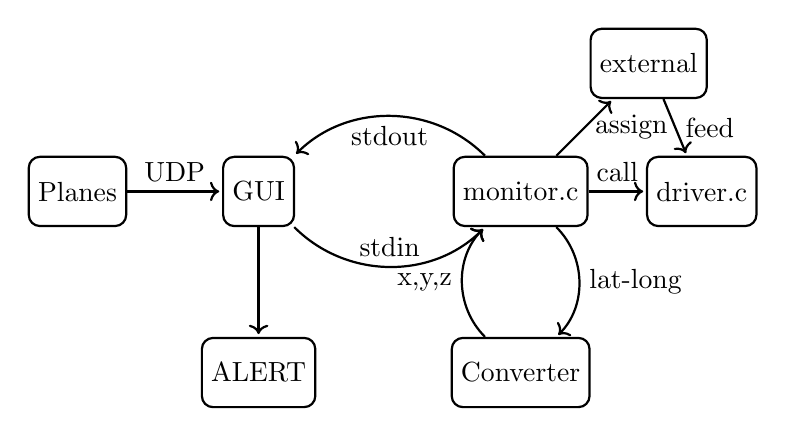
\begin{tikzpicture}[->, node distance=2.3cm, auto, shorten >=1pt, bend angle=45,thick]
		\tikzstyle{every state}=[rectangle, rounded corners]
		
		\node[state] (Plane) {Planes};
		\node[state] (GUI) [right of=Plane] {GUI};
		\node[state] (Mon) [right=2cm of GUI] {monitor.c};
		\node[state] (dr) [right of=Mon] {driver.c};
		\node[state] (ex) [above right of=Mon] {external};
		
		
		\node[state] (AL) [below of=GUI] {ALERT};
		\node[state] (Co) [below of=Mon] {Converter};
		
		
		\tikzstyle{every node}=[]
		
		
		\path
		(Plane) edge node {UDP} (GUI)
		(GUI) edge [bend right] node {stdin} (Mon)
		(Mon) edge [bend right] node {stdout} (GUI)
		(Mon) edge [bend left, anchor=west] node {lat-long} (Co)
		(Co) edge [bend left, anchor=west] node[left] {x,y,z} (Mon)
		(Mon) edge [anchor=west] node {assign} (ex)
		(Mon) edge [anchor=south] node {call} (dr)
		(ex) edge [anchor=west] node {feed} (dr)
		(GUI) edge node {} (AL);
		\end{tikzpicture}
	\end{figure}
\end{frame}

\begin{frame}
	\frametitle{What's next ?}
	\begin{enumerate}
		\item Code refactoring, writing documentation
		\item Add more cases for unit testing of WCV
		\item Test the WCV in a real situation (fall 2015)
		\item Find other new applications
		\item Develop new libraries (matrix, math functions)
		\item Reimplement the QuickCheck for SBV backend
		\item Submit a paper
		\item goto 1:
	\end{enumerate}
\end{frame}

\begin{frame}
	\frametitle{Questions}
	\text{Questions ?}
\end{frame}
  	
\end{document}
